% !Mode:: "TeX:UTF-8"
\documentclass[17pt]{beamer}
\usepackage[adobefonts]{ctex}
\usepackage{graphicx}
\usepackage{tabularx}
\usepackage{fix-cm}
\usepackage{color}

\definecolor{title}{RGB}{128,128,128}

\setlength{\paperwidth}{25.4cm}
\setlength{\paperheight}{19.05cm}
\setlength{\textwidth}{.95\paperwidth}
\setlength{\textheight}{\paperheight}

\newcommand{\zihaopt}[2]{\fontsize{#1}{\baselineskip}\selectfont#2}

\setCJKmainfont{SimSun}
\setsansfont{Times New Roman}

\setCJKfamilyfont{xinwei}{STXinwei}
\newcommand{\xinwei}[1]{{\CJKfamily{xinwei}#1}}
\setCJKfamilyfont{hei}{SimHei}
\newcommand{\hei}[1]{{\CJKfamily{hei}#1}}

\setbeamertemplate{navigation symbols}{}

\newcommand{\tutor}[1]{\setbeamertemplate{tutor}{#1}}
\newcommand{\sid}[1]{\setbeamertemplate{sid}{#1}}

% 需要修改的全局变量
\title{数学公式检索系统的设计与实现}
\sid{38211214}
\author{扈\quad 煊}
\tutor{杜孝平}
\institute{北大计算机所}

\setbeamertemplate{title page}{
    \vspace{1cm}

    {
        \setlength{\extrarowheight}{2cm}
        \begin{tabularx}{\textwidth}{@{\hspace{1.75cm}}X}
            \textcolor{title}{\xinwei{\zihaopt{44}{本科生毕设设计答辩}}} \\
            \bf{\textcolor{blue}{\zihaopt{28}{\inserttitle}}} \\
        \end{tabularx}
    }

    \vspace{1.98cm}

    \hei{\zihaopt{31}{
        \setlength{\extrarowheight}{0.3cm}
        \begin{tabularx}{\textwidth}{@{\hspace{3.2cm}}ccc}
            \makebox[6cm]{学\hfill 号} & : & \makebox[7cm]{\hfill \usebeamertemplate{sid} \hfill} \\
            \makebox[6cm]{姓\hfill 名} & : & \makebox[7cm]{\hfill \insertauthor \hfill}\\
            \makebox[6cm]{指\hfill 导\hfill 教\hfill 师}  & :& \makebox[7cm]{\hfill \usebeamertemplate{tutor} \hfill} \\
            \makebox[6cm]{实\hfill 习\hfill 单\hfill 位}  & :& \makebox[7cm]{\hfill \insertinstitute \hfill} \\
        \end{tabularx}
    }}
}

\setbeamertemplate{itemize items}[square]
\setbeamertemplate{itemize subitem}[circ]
\setbeamerfont{itemize/enumerate body}{size*={28}{\baselineskip}}
\setbeamerfont{itemize/enumerate subbody}{size*={24}{\baselineskip}}

\setbeamertemplate{section in toc}[square]
\setbeamercolor{section in toc}{fg=black}
\setbeamerfont{section in toc}{size*={28}{\baselineskip},series=\bfseries}

\setbeamertemplate{frametitle}{\vspace{2cm}\hspace{0.8cm}\insertframetitle}
\setbeamercolor{frametitle}{fg=blue}
\setbeamerfont{frametitle}{size*={44}{\baselineskip},series=\bfseries}

\setbeamertemplate{bibliography item}{\insertbiblabel}
\setbeamercolor{bibliography item}{fg=black}
\setbeamercolor{bibliography entry author}{fg=black}


\begin{document}
\CTEXnoindent

    \usebackgroundtemplate{
        
\includegraphics[width=\paperwidth,height=\paperheight]{pic/bg1.png}
    } % 第一页背景 

    \frame{\titlepage}

    \usebackgroundtemplate{
        
\includegraphics[width=\paperwidth,height=\paperheight]{pic/bg2.png}
    } % 其它页背景

    % 提纲页,用目录方式生成
    \begin{frame}
        \frametitle{汇报内容}
        \tableofcontents
    \end{frame}

    % Slide主要内容的开始

    \section{背景、意义与研究现状} % Section名称用于生成目录 
    
    \begin{frame}
        \frametitle{背景、意义与研究现状} % 标题
        \begin{columns} % 分栏
            \pause % 暂停,实现动画效果

            \column{.5\textwidth} % 第一栏    
            \begin{itemize} % 列表
                \item 基于文本检索
                \item 基于树状结构的检索
                \begin{itemize} % 列表嵌套(子列表)
                    \item 基于替代树索引
                    \item 基于路径索引
                \end{itemize}
            \end{itemize}

            \pause

            \column{.5\textwidth}    
            \begin{itemize}
                \item Wolfram MathWorld
                \item LaTeX Search
                \item Mathdex
                \item ActiveMath
                \item MathWebSearch
            \end{itemize}

        \end{columns}
    \end{frame}
    
    \section{相关原理与技术}
    
    \begin{frame}
        \frametitle{相关原理与技术}
        
        \begin{itemize}
          \item<2-> 搜索引擎 % 箭括号实现显示顺序的动画
          \item<4-> MathML
          \begin{itemize}
            \item<4-> Content MathML
            \item<4-> Presentation MathML
          \end{itemize}
          \item<3-> MongoDB
        \end{itemize}
    \end{frame}

    \begin{frame}
        \frametitle{相关原理与技术 --- MathML(1)}
        \begin{center} % 图片,居中
            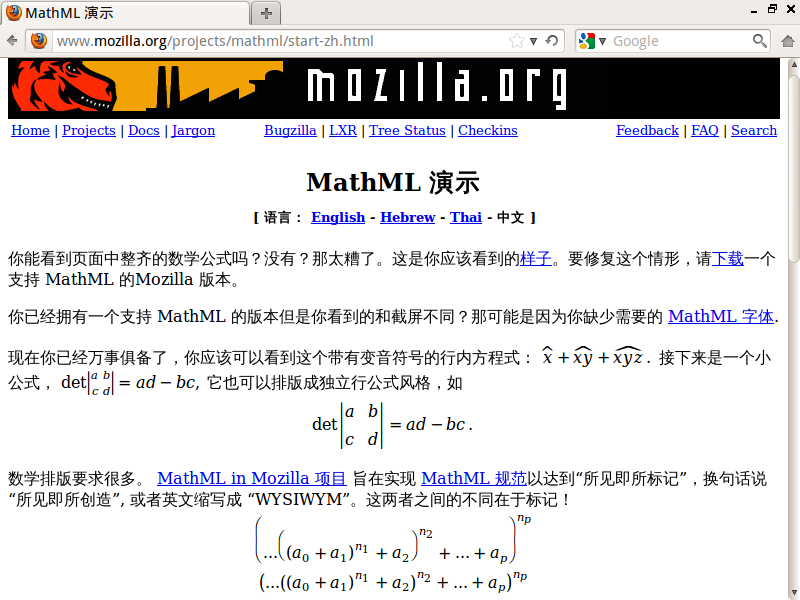
\includegraphics[width=0.8\textwidth]{pic/mathml1.png}
        \end{center}
    \end{frame}
    
    \begin{frame}
        \frametitle{相关原理与技术 --- MathML(2)}
        \begin{center}
            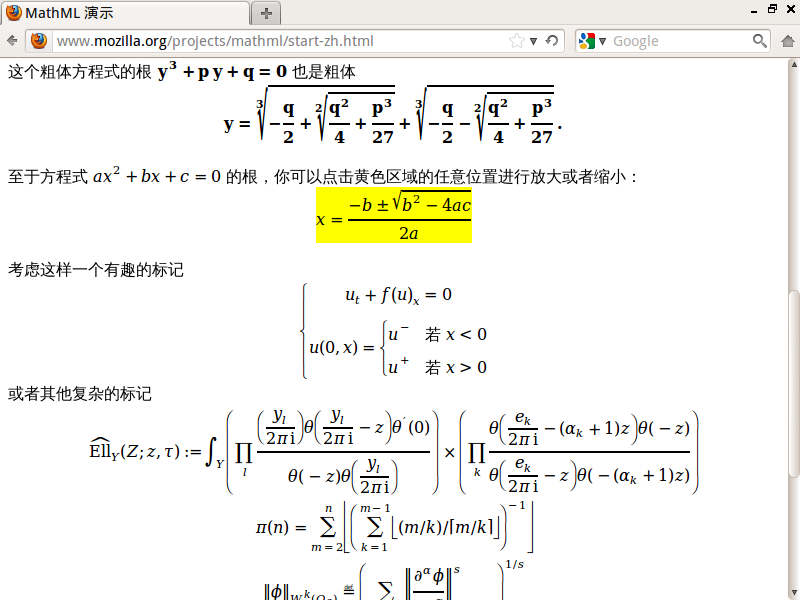
\includegraphics[width=0.8\textwidth]{pic/mathml2.png}
        \end{center}
    \end{frame}
    
    \section{系统设计与实现}
    
    \begin{frame}
        \frametitle{系统设计}
        \vspace{-5cm} % 垂直距离的HACK
        \begin{columns}
            \column{0.5\textwidth}
                \begin{center}
                    \begin{itemize}
                        \item 黑色为离线部分
                        \item[] 索引建立 % 实现没有标记的列表项
                        \item 蓝色为在线部分
                        \item[] 查询处理
                    \end{itemize}
                \end{center}
            \column{0.5\textwidth}
                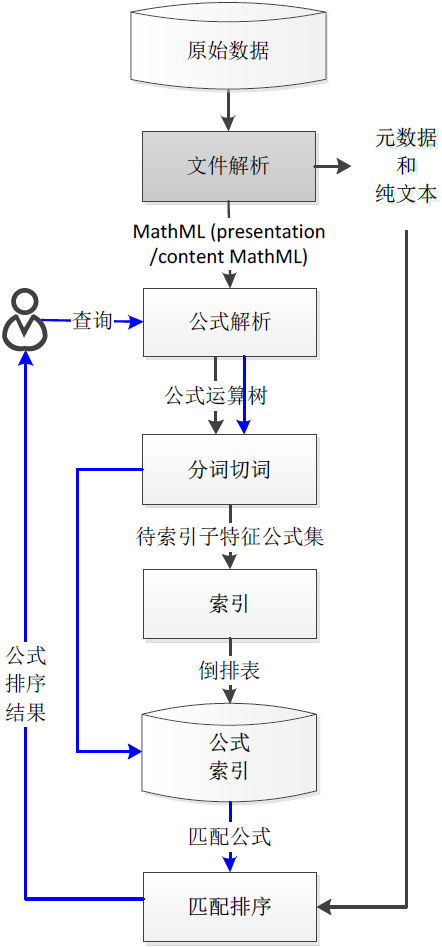
\includegraphics[height=0.8\textheight]{pic/process.png}
        \end{columns}
    \end{frame}

    \begin{frame}
        \frametitle{系统实现}
        \begin{columns}
            \column{0.5\textwidth}
                \begin{itemize}
                    \item 文件解析
                    \item 公式解析
                    \item 分词切词
                    \item 公式索引
                    \item 匹配排序
                \end{itemize}
            \column{0.5\textwidth}
                \begin{itemize}
                    \item 分词切词
                    \begin{itemize}
                        \item 归一化
                        \item 切词
                        \item 泛化
                    \end{itemize}
                \end{itemize}
        \end{columns}
    \end{frame}
    
    \section{系统测试与评估}
    
    \begin{frame}
        \frametitle{系统测试---索引}
        \begin{itemize}
            \item 文档数 181篇
            \item 数学公式 61591个
            \item 时间 35分钟
            \item 数据库
            \begin{itemize}
                \item 数据空间 236,353,804 字节
                \item 索引空间 119,950,096 字节
            \end{itemize}
        \end{itemize}
    \end{frame}

    \begin{frame}
        \frametitle{系统测试---首页}
        \begin{center}
            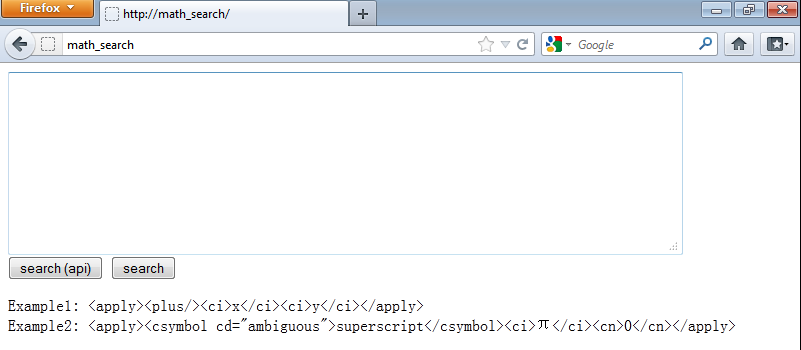
\includegraphics[width=.8\paperwidth]{pic/test_index.png}
        \end{center}
    \end{frame}

    \begin{frame}
        \frametitle{系统测试---测试1}
        \begin{center}
            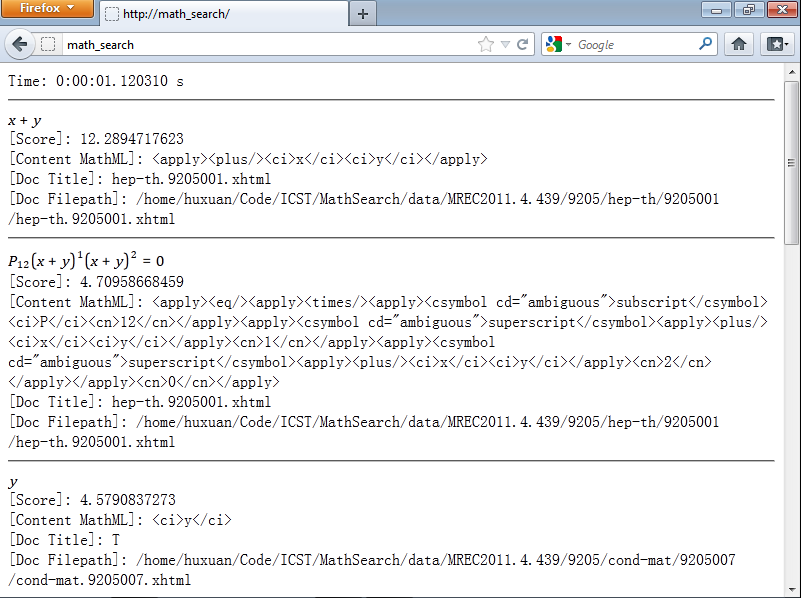
\includegraphics[width=.7\paperwidth]{pic/test1.png}
        \end{center}
    \end{frame}

    \begin{frame}
        \frametitle{系统测试---测试1(API)}
        \begin{center}
            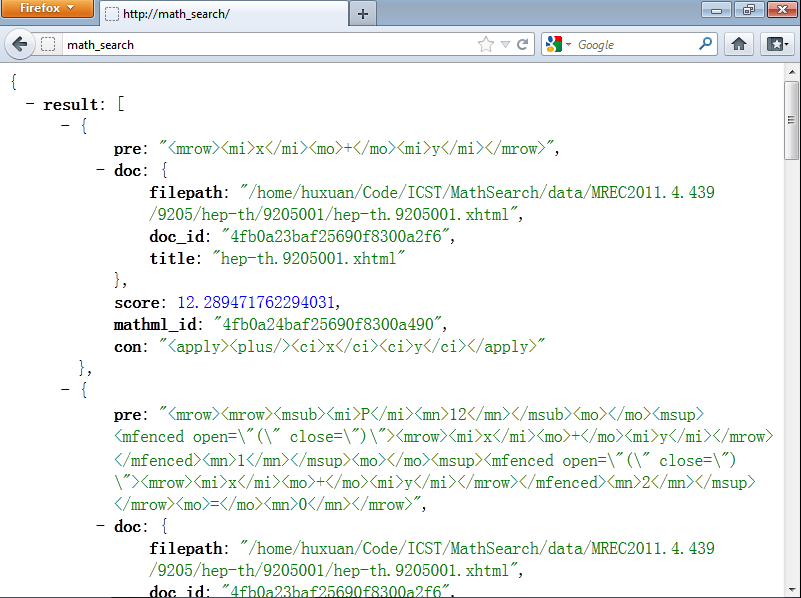
\includegraphics[width=.7\paperwidth]{pic/test1_api.png}
        \end{center}
    \end{frame}

    \begin{frame}
        \frametitle{系统测试---测试2}
        \begin{center}
            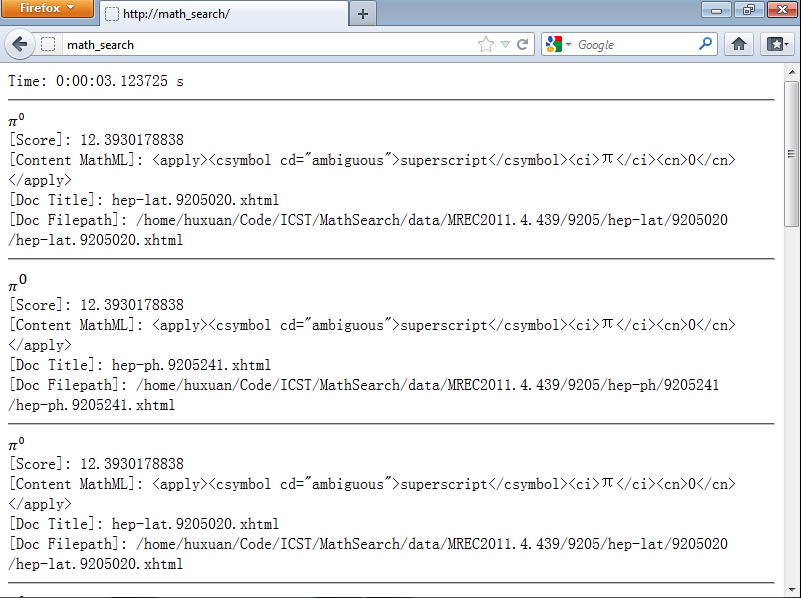
\includegraphics[width=.7\paperwidth]{pic/test2.png}
        \end{center}
    \end{frame}

    \begin{frame}
        \frametitle{系统测试---测试2(API)}
        \begin{center}
            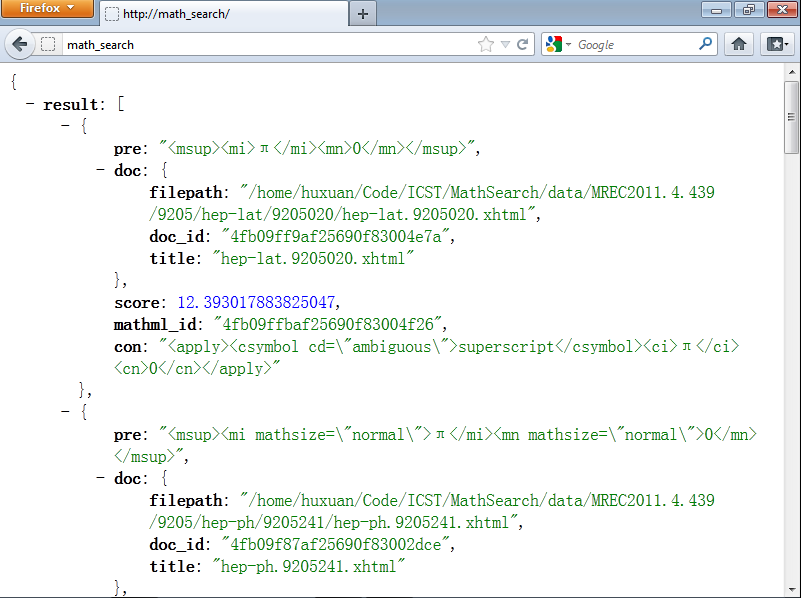
\includegraphics[width=.7\paperwidth]{pic/test2_api.png}
        \end{center}
    \end{frame}

    \begin{frame}
        \frametitle{系统评估}
        \begin{itemize}
            \item 匹配 - tf 和 idf
            \item 泛化 - 类似表达式
            \item 模糊化 - 子/母表达式
        \end{itemize}
    \end{frame}
    
    \section{总结展望}
    
    \begin{frame}
        \frametitle{总结展望}
        \vspace{-3cm}
        \begin{columns}
            \column{.35\textwidth}
                \begin{itemize}
                    \item 总结
                    \begin{itemize}
                        \item 基本框架
                        \item 原始数据的解析
                        \item 数学公式的解析
                        \item[] 子特征表达式
                        \item 索引的匹配排序
                    \end{itemize}
                \end{itemize}

            \pause

            \column{.65\textwidth}
                \begin{itemize}
                    \item 展望
                    \begin{itemize}
                        \item 索引存储
                        \item 数据格式
                        \item[] LaTeX 和 Presentation MathML
                        \item 子特征表达式的生成算法
                        \item 查询条件输入方式
                        \item 检索结果输出方式
                        \item 原始数据
                        \item[] 维基百科
                    \end{itemize}
                \end{itemize}
        \end{columns}
    \end{frame}
    
    \section{参考文献}
    
    \begin{frame}
        \frametitle{参考文献}
        \vspace{-1.5cm}
        \begin{thebibliography}{} % 参考文献,目前未支持bib,直接拷贝原文,方括号中的序号即为显示的序号
            \bibitem[1]{1} W. B. Croft, D. Metzler, T. Strohman. Search Engines: Information Retrieval in Practice [M]. USA: Addison-Wesley Publishing Company, 2009, 1-552.
            \bibitem[2]{2} A. Ron, B. Stephen, C. David, et al. Mathematical Markup Language (MathML) Version 3.0 [R]. W3C Recommendation , World Wide Web Consortium (W3C) 2010.
            \bibitem[3]{3} P. Sojka, M. Lí?ka. The Art of Mathematics Retrieval [A]. the 11th ACM Symposium on Document Engineering (DocEng '11) [C]. New York, USA: ACM, 2011: 57-60.
            \bibitem[4]{4} J. Zhao, M. Y. Kan, and Y. L. Theng. Math information retrieval: user requirements and prototype implementation [A]. The 8th ACM/IEEE-CS Joint Conference on Digital Libraries (JCDL '08) [C], New York, NY, USA: ACM, 2008: 187-196.
            \bibitem[5]{5} B. R. Miller, A. Youssef. Technical Aspects of the Digital Library of Mathematical Functions [J]. Annals of Mathematics and Artificial Intelligence, 2003, 38(1): 121–136.
        \end{thebibliography}
    \end{frame}

    \begin{frame}
        \frametitle{参考文献(续)}
        \vspace{-1.5cm}
        \begin{thebibliography}{}
            \bibitem[6]{6} A. Youssef,  Search of Mathematical Contents: Issues And Methods [A]. The ISCA 14th International Conference on Intelligent and Adaptive Systems and Software Engineering (IASSE '05) [C], Toronto, Canada: ISCA, 2005: 100-105.
            \bibitem[7]{7} P. Libbrecht, E. Melis. Methods to Access and Retrieve Mathematical Content in ACTIVEMATH [A]. the 2nd International Conference on Mathematical Software (ICMS'06) [C]. Castro Urdiales, Spain: Springer-Verlag, 2006: 331-342.
            \bibitem[8]{8} R. Miner, R. Munavalli. An Approach to Mathematical Search Through Query Formulation and Data Normalization [A]. The 14th Symposium on Towards Mechanized Mathematical Assistants: 6th International Conference (Calculemus '07 / MKM '07) [C]. Hagenberg, Austria: Springer-Verlag, 2007: 342-355.
            \bibitem[9]{9} A. Youssef. Relevance Ranking and Hit Description in Math Search [J]. Mathematics in Computer Science, 2008, 2(2): 333-353.
        \end{thebibliography}
    \end{frame}

    \begin{frame}
        \frametitle{参考文献(续)}
        \vspace{-1.5cm}
        \begin{thebibliography}{}
            \bibitem[10]{10} A. Youssef. Methods of Relevance Ranking and Hit-content Generation in Math Search [A]. The 14th Symposium on Towards Mechanized Mathematical Assistants: 6th International Conference (Calculemus '07 / MKM '07) [C]. Hagenberg, Austria: Springer-Verlag, 2007: 393-406.
            \bibitem[11]{11} M. Altamimi, A. Youssef. A Math Query Language with an Expanded Set of Wildcards [J]. Mathematics in Computer Science, 2008, 2(2): 305-331.
            \bibitem[12]{12} M. Kohlhase, I. Sucan. A Search Engine for Mathematical Formulae [M]. Artificial Intelligence and Symbolic Computation. Berlin, Heidelberg: Springer, 2006: 241-253.
            \bibitem[13]{13} S. Kamali, F. W. Tompa. A new mathematics retrieval system [A]. The 19th ACM International Conference on Information and Knowledge Management (CIKM '10) [C]. Toronto, ON, Canada: ACM, 2010: 1413-1416.
            \bibitem[15]{15} S. Kamali and F. W. Tompa. Improving Mathematics Retrieval [J]. Towards a Digital Mathematics Library, 2009: 37-48.
        \end{thebibliography}
    \end{frame}

    \begin{frame}
        \frametitle{参考文献(续)}
        \vspace{-1.5cm}
        \begin{thebibliography}{}
            \bibitem[14]{14} Y. Hijikata, H. Hashimoto, S. Nishida. Search Mathematical Formulas by Mathematical Formulas [A]. The Symposium on Human Interface 2009 on ConferenceUniversal Access in Human-Computer Interaction. Part I: Held as Part of HCI International 2009 [C]. San Diego, CA: Springer-Verlag, 2009: 404-411.
            \bibitem[16]{16} R. Zanibbi, B. Yuan. Keyword and Image-based Retrieval of Mathematical Expressions [A]. Document Recognition and Retrieval XVIII  (DRR '11) [C].  San Francisco, California, USA: SPIE, 2011: 78740I-9.
            \bibitem[17]{17} C. David. An introduction to MathML [DB/OL]. http://www.ibm.com/developerworks/xml/library/x-mathml3/, 2009-12-15/2012-05-25.
            \bibitem[18]{18} H. Tony, Introduction - MongoDB [DB/OL]. http://www.mongodb.org/display/docs/Introduction/, 2011-09-15/2012-05-25.
            \bibitem[19]{19} C. Kristina, D. Michael. MongoDB: The Definitive Guide [M]. USA: O’Reilly Media, 2010: 1-193.
        \end{thebibliography}
    \end{frame}

    % Slide主要内容的结束
    % 最后一页自动生成

    \begin{frame}
        \vspace{4cm}
    
        \bf \zihaopt{60}{
            \begin{tabularx}{\textwidth}{c}
                \makebox[\textwidth]{\hfill \color{blue}{敬请批评指正!} \hfill}
            \end{tabularx}
        }
        
        \vspace{1cm}
        
        \bf \zihaopt{24}{
            \setlength{\extrarowheight}{-3cm}
            \begin{tabularx}{\textwidth}{@{\hspace{6cm}}ccc}
                \makebox[4cm]{学\hfill 号} & : & \makebox[4cm]{\hfill \usebeamertemplate{sid} \hfill} \\
                \makebox[4cm]{姓\hfill 名} & : & \makebox[4cm]{\hfill \insertauthor \hfill} \\
            \end{tabularx}
        }
    \end{frame}
\end{document}
